\subsubsection{Rancangan Detail Subsistem Kontrol}
\label{subsubsection:detail-subsistem-kontrol}
  
Subsistem Kontrol bertanggung jawab mengelola transaksi dan konsistensi antar-\textit{Node}. Pengelolaan tersebut dilakukan dengan mengaplikasikan algoritma konsensus untuk menjaga konsistensi data antar-\textit{Node}. Subsistem ini juga bertanggung jawab untuk melakukan \textit{recovery} data dari \textit{transaction log} jika terjadi kegagalan pada \textit{Node}.

Ilustrasi struktur subsistem kontrol dapat dilihat pada gambar \ref{fig:control-subsystem-structure}.

% _TODO: Change image
\begin{figure}[ht]
    \centering
    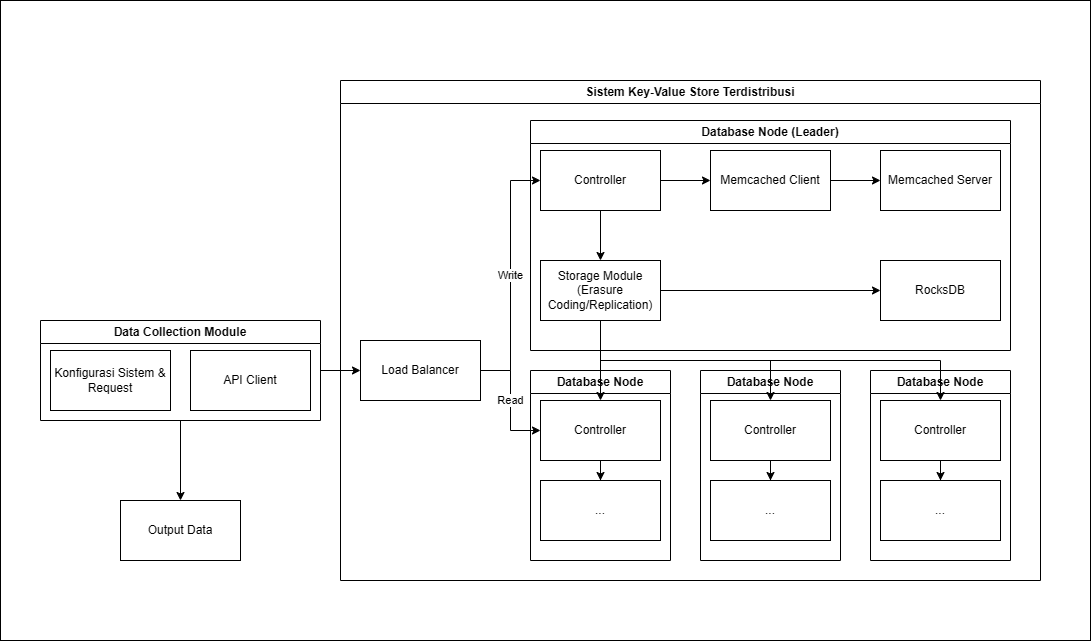
\includegraphics[width=0.95\textwidth]{resources/chapter-3/general-architecture.png}
    \caption{Struktur Subsistem Kontrol}
    \label{fig:control-subsystem-structure}
\end{figure}